\begin{frame}

\begin{center}

\Huge \textbf{DEMO}

\bigskip

\large Look at that "file"!

\end{center}

\end{frame}

\begin{frame}

\frametitle{DEMO: TFS Overview}

\begin{center}

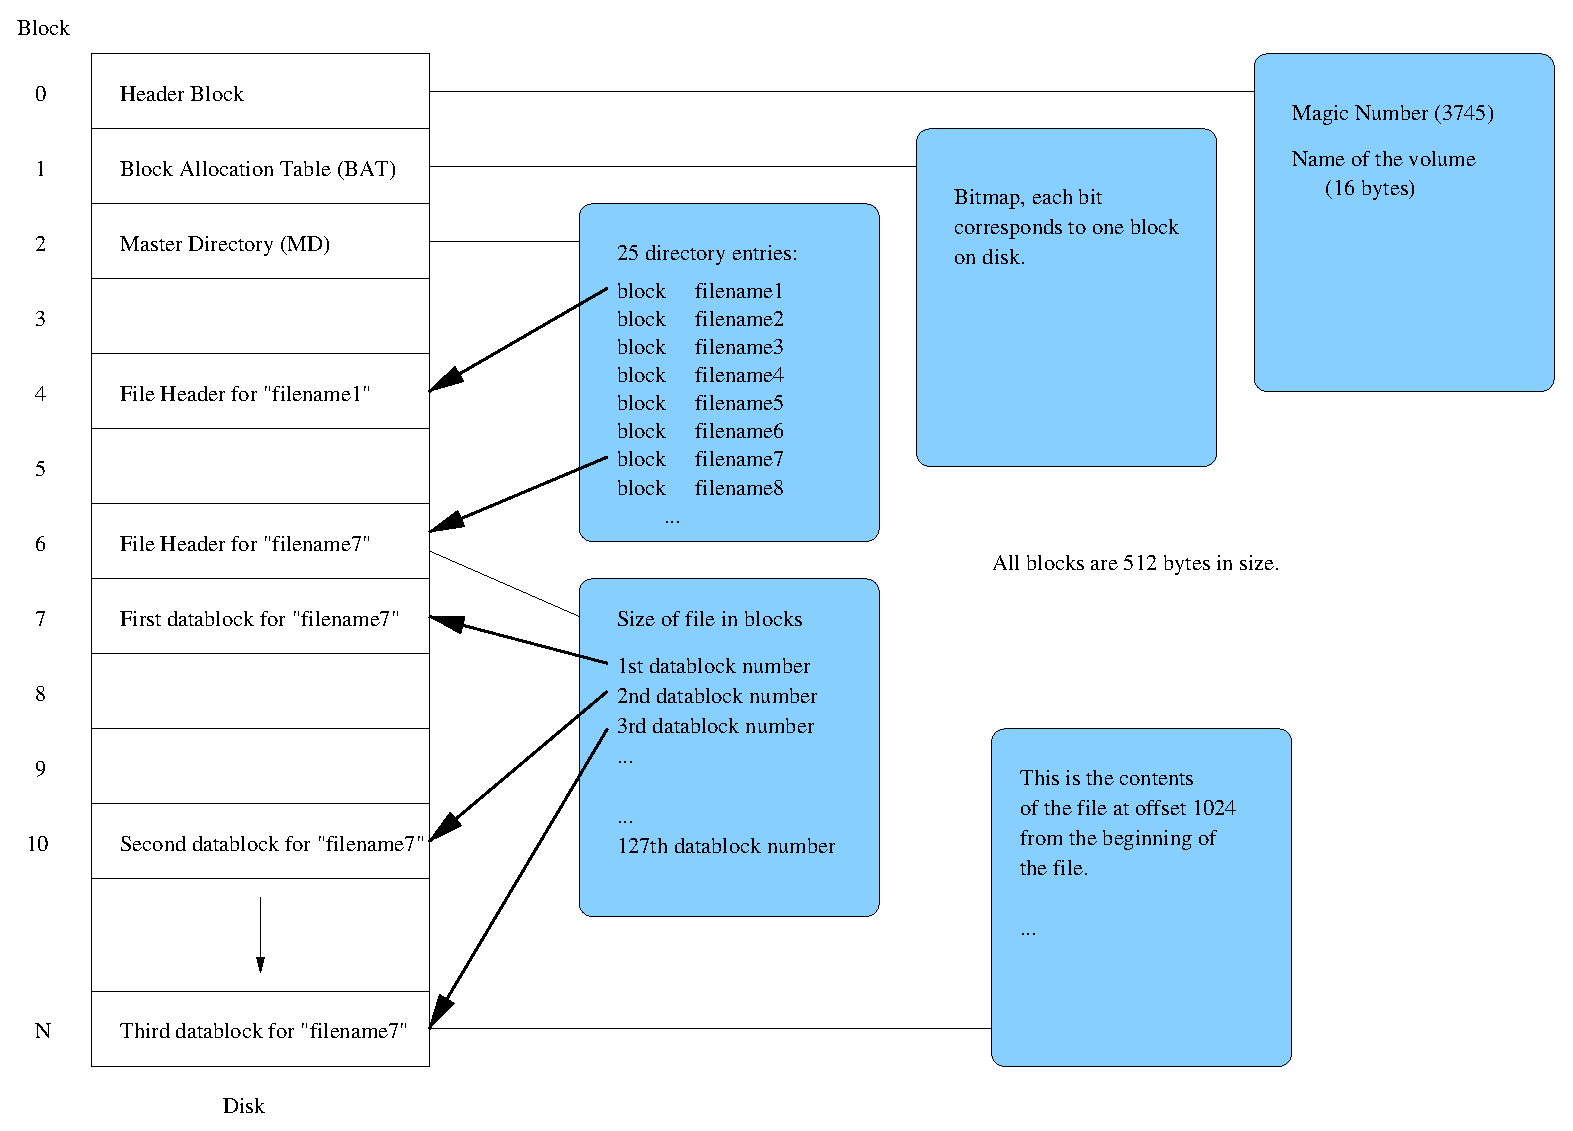
\includegraphics[width=\textwidth]{figures/tfs}

\end{center}

\end{frame}


\begin{frame}[fragile]

\frametitle{DEMO: Log (1/3)}

\begin{itemize}

\item All blocks in TFS are 512 bytes; the first block is 4-bytes magic number,
16 bytes volume name, the rest is wasted:

\begin{verbatim}
union header {
  struct {
    uint32_t magic;
    char volname[16];
  };
  uint8_t padding[512];
} header;
\end{verbatim}

\item TFS is big-endian, my machine (x86\_64) is little-endian:

\begin{verbatim}
uint2_t from_big_endian(uint32_t value) {
  return ((value & 0xFF000000) >> 24) |
         ((value & 0x00FF0000) >> 8)  |
         ((value & 0x0000FF00) << 8)  |
         ((value & 0x000000FF) << 24);
}
\end{verbatim}

\end{itemize}

\end{frame}


\begin{frame}[fragile]

\frametitle{DEMO: Log (2/3)}

Use (userland) buffered I/O:

\begin{verbatim}
FILE *stream;
size_t read;
int retval;
...
stream = fopen("store.file", "r");
...
read = fread(&header, sizeof(union header), 1, stream);
...
retval = fclose(stream);
\end{verbatim}

\end{frame}


\begin{frame}[fragile]

\frametitle{DEMO: Log (3/3)}

\begin{columns}[T]

\begin{column}[T]{.45\textwidth}

\begin{itemize}

\item See attached \texttt{tfs.c}:

\begin{verbatim}
$ make tfs
cc     tfs.c   -o tfs
$ ./tfs 
Magic number: ea1
Volume name: disk
\end{verbatim}

\end{itemize}

\end{column}

\begin{column}[T]{.55\textwidth}

\begin{itemize}

\item See attached \texttt{fat32.c}:

\begin{verbatim}
$ make fat32
cc     fat32.c   -o fat32
$ ./fat32
jmpboot: eb5890
oemname: mkfs.fat
bytes_per_sec: 258
sec_per_clus: 32 
\end{verbatim}

\end{itemize}

\end{column}

\end{columns}

\vspace{\fill}

\begin{itemize}

\item You could even modify \texttt{fat32.c} to read \texttt{"/dev/sdb1"}
instead of \texttt{"fatdisk"} --- this is how \texttt{mount} works.

\item For more details on FAT, see:

\begin{quote}

\footnotesize Microsoft Corporation, FAT: General Overview of On-Disk Format,
Version 1.03, December 6, 2000. \url{http://www.webcitation.org/6g0OHfQxp}

\end{quote}

\end{itemize}

\end{frame}
